\documentclass[12pt]{article}
\usepackage[a4paper, margin=1in]{geometry}
\usepackage{amsmath}
\usepackage{amssymb}
\usepackage{amsthm}
\usepackage{amsfonts}
\usepackage{tabularx}
\usepackage{graphicx}
\newcounter{questionnumber}
\newenvironment{question}[1][]{\stepcounter{questionnumber}\par\noindent\textbf{Question \thequestionnumber. #1}\par}{\par}
\newenvironment{solution}{\par\noindent\textbf{Solution:}\par}{\par\vspace{1em}}
\begin{document}
\section{Discussion 02a}
\begin{question}
    \noindent
    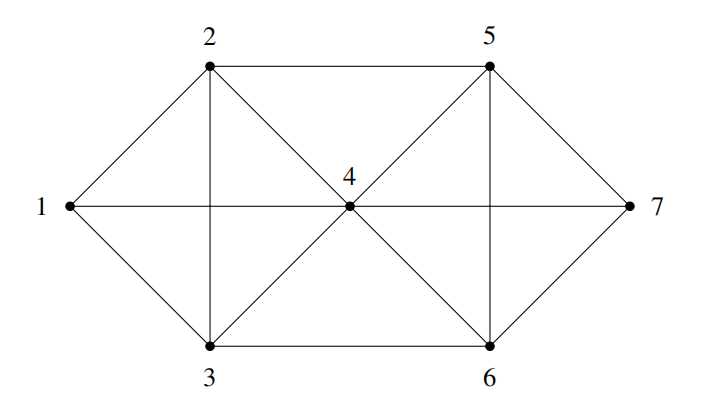
\includegraphics[width=0.5\textwidth]{graph1.png}\\
    (a) Is there an Eulerian tour in the graph above? If no, give justification. If yes, provide an example.\\
    (b) Is there an Eulerian walk in the graph above? An Eulerian walk is a walk that uses each edge exactly once. If no, give justification. If yes, provide an example.\\
    (c) What is the condition that there is an Eulerian walk in an undirected graph? Briefly justify your answer.
\end{question}
\begin{solution}
    \noindent
    (a) No. The vertex 1 has odd degree.\\
    (b) Yes. 1-2-4-1-3-2-5-6-3-4-5-7-4-6-7.\\
    (c) Either the connected(except for isolated vertices) graph has even degree or there are exactly two vertices with odd degree.
    If all vertices have even degree, then there exists an Eulerian tour, therefore an Eulerian walk exists.
    If there are exactly two vertices with odd degree, we can set these two vertices as the starting point and the end point.
\end{solution}
\begin{question}
    \noindent
    (a) Prove that all trees with at least 2 vertices have at least two leaves. Recall that a leaf is defined as a node in a tree with degree exactly 1.\\
    (b) Prove that all trees with at least 2 vertices are \emph{bipartite}: the vertices can be partitioned into two groups so that every edge goes between the two groups.

    [Hint: Use induction on the number of vertices.]
\end{question}
\begin{solution}
    \noindent
    (a) Find a leaf first. Then set the starting point at the leaf and find a path to another leaf. Therefore, we have found 2 leaves.\\
    (b) It's trivial when there are exactly 2 vertices. Assume that all trees with $n$ vertices are bipartite.
    For any tree with $n+1$ vertices, remove a leaf and the edge connected to it, and the graph left is a tree with $n$ vertices, which is bipartite according to the assumption.
    Then, add the leaf back have it into the different group from the vertex connected to it. Therefore, we have partitioned all the $n+1$ vertices into 2 groups so that every edge goes between the two groups.
\end{solution}
\begin{question}
    The degree sequence of a graph is the sequence of the degrees of the vertices, arranged in descending order, with repetitions as needed. For example, the degree sequence of the following graph is (3,2,2,2,1).

    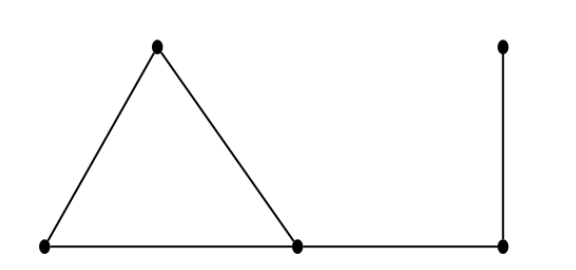
\includegraphics[width=0.5\textwidth]{graph2.png}

    For each of the parts below, determine if there exists a simple undirected graph G (i.e. a graph without self-loops and multiple-edges) having the given degree sequence. Justify your claim.\\
    (a) (3,3,2,2)\\
    (b) (3,2,2,2,2,1,1)\\
    (c) (6,2,2,2)\\
    (d) (4,4,3,2,1)\\
\end{question}
\begin{solution}
    \noindent
    (a) There exists $\mathrm{G}(V,E)$ such that $V=\{A,B,C,D\}$, $E=\{\{A,B\},\{A,C\},\{A,D\},\{B,C\},\{B,D\}\}$\\
    (b) Does not exist. $2E=3+2+2+2+2+1+1=13$, which is impossible for any integer $E$.\\
    (c) Does not exist. It is impossible to have degree 6 since there is only 4 vertices.\\
    (d) Does not exist. Having 2 vertices with degree 4 means that these 2 vertices are connected with every other vertex. Therefore, it is impossible to have a vertex with degree 1, since it is connected with those two vertices.
\end{solution}
\section{Discussion 02b}
\begin{question}
    In each part below, provide the number/equation and brief justification.\\
    (a) A connected planar simple graph has 5 more edges than it has vertices. How many faces does it have?\\
    (b) How many edges need to be removed from a 3-dimensional hypercube to get a tree?\\
    (c) The Euler's formula $v - e + f = 2$ requires the planar graph to be connected. What is the analogous formula for planar graphs with $k$ connected components?
\end{question}
\begin{solution}
    \noindent
    (a) $v-\left( v+5 \right) +f=2\Longrightarrow f=7$\\
    (b) $8-e+1=2\Longrightarrow e=7$, $12-7=5$\\
    (c) $v-e+\left( f+k-1 \right) =2k\Longrightarrow v-e+f=k+1$
\end{solution}
\begin{question}
In each part below, you are given some information about a graph G. Using only the information in the current part, say whether G will always be planar, always be non-planar, or could be either. If you think it is always planar or always non-planar, prove it. If you think it could be either, give a planar example and a non-planar example.\\
(a) G can be vertex-colored with 4 colors.\\
(b) G requires 7 colors to be vertex-colored.\\
(c) $e \leq 3v - 6$, where $e$ is the number of edges of G and $v$ is the number of vertices of G.\\
(d) G is connected, and each vertex in G has degree at most 2.\\
(e) Each vertex in G has degree at most 2.
\end{question}
\begin{solution}
    \noindent    
    (a) Either. A 4-vertices graph can always be colored with 4 colors. $K_{3,3}$ can be colored where all houses are the same color and all wells are the same color. \\
    (b) Non-planar. Because every planar graph can be colored with 5 colors.\\
    (c) Either. A triangle is planar and a $K_{3_3}$ is non-planar.\\
    (d) Planar. Either $K_{3,3}$ or $K_5$ has vertices with degree more than 2.\\
    (e) Planar. Because its each connected component is planar.
\end{solution}
\begin{question}
    $\text{Prove that a graph with maximum degree at most }k\mathrm{~is~}(k+1)\text{-colorable.}$
\end{question}
\begin{solution}
    When there is only 1 vertex, it is trivial.
    Assume that the statement holds true for any graph with $n$ vertices.
    For any graph with $(n+1)$ vertices, delete one random vertex and the edges connected to it, then color the $n$ vertices left with $(k+1)$ colors.
    Then, add the vertex and edges back, since there are at most $k$ vertices connected to it, there is at least one color left for this vertex.
    Color the vertex, and we get this graph with $(n+1)$ vertices with at most $(k+1)$ colors, which means it is $(k+1)$-colorable.
    Therefore, we have proven that for any graph with maximum degree at most $k$ is $(k+1)$-colorable.
\end{solution}
\begin{question}
    The vertex set of the n-dimensional hypercube G = (V,E) is given by V = $\{0,1\}^n$ (recall that $\{0,1\}^n$ denotes the set of all n-bit strings). There is an edge between two vertices x and y if and only if x and y differ in exactly one bit position.\\
    (a) Draw 1-, 2-, and 3-dimensional hypercubes and label the vertices using the corresponding bit strings.\\
    (b) Show that the edges of an n-dimensional hypercube can be colored using n colors so that no pair of edges sharing a common vertex have the same color.\\
    (c) Show that for any $n\geq1$, the n-dimensional hypercube is bipartite.
\end{question}
\begin{solution}
    \noindent
    (a) \\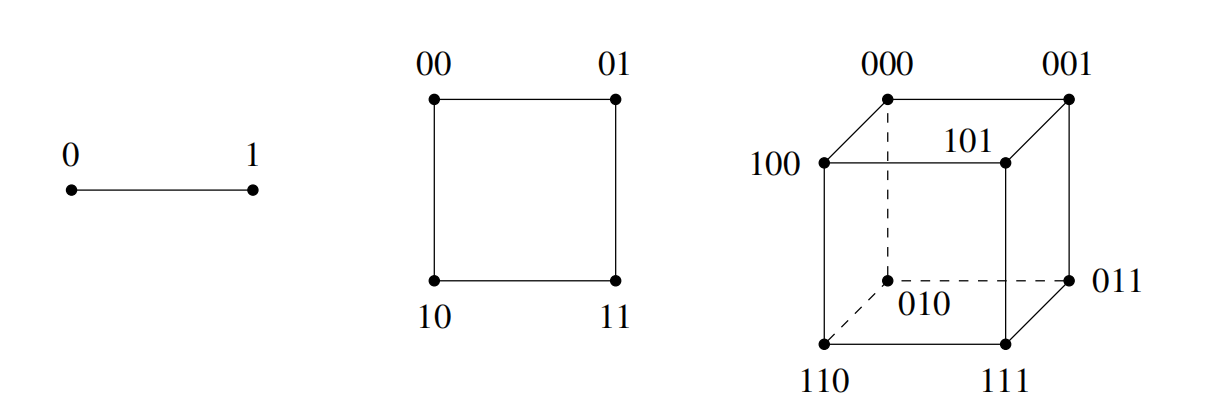
\includegraphics[width=0.5\textwidth]{graph3.png}\\
    (b) For an 1-dimensional hypercube, it is trivial.
    Assume that the statement is true for the $n$-dimensional hypercube.
    For an $(n+1)$-dimensional hypercube, the vertices $0x$ and the edges between them form a $n$-dimensional hypercube.
    Similarly, the vertices $1x$ and the edges between form a $n$-dimensional hypercube too. Color the edges in these two hypercubes with the same $n$ colors.
    Color all edges between $0x$ and $1x$ with a different color from the previous $n$ colors, then we finish coloring the $(n+1)$-dimensional hypercube with $(n+1)$ colors.\\
    (c) For every vertex, add up all the bits together. If the sum is odd then the vertex is in group 1, otherwise the vertex is in group 0.
    Every 2 vertices share the same edge differ in exactly on bit position, so they are in different groups, therefore the hypercube is bipartite.
\end{solution}
\section{Homework 02}
\begin{question}
    What is wrong with the following "proof"? In addition to finding a counterexample, you should explain what is fundamentally wrong with this approach, and why it demonstrates the danger of build-up error.\\
    \textbf{False Claim:} If every vertex in an undirected graph has degree at least 1,then the graph is connected.\\
    \textit{Proof?} We use induction on the number of vertices $n\geq1.$\\
    \textit{Base case:} There is only one graph with a single vertex and it has degree $0.$ Therefore, the base case is vacuously true, since the if-part is false.\\
    \textit{Inductive hypothesis:} Assume the claim is true for some $n\geq 1.$\\
    \textit{Inductive step:} We prove the claim is also true for $n+1.$ Consider an undirected graph on $n$ vertices in which every vertex has degree at least 1. By the inductive hypothesis, this graph is connected. Now add one more vertex $x$ to obtain a graph on $(n+1)$ vertices, as shown below.

    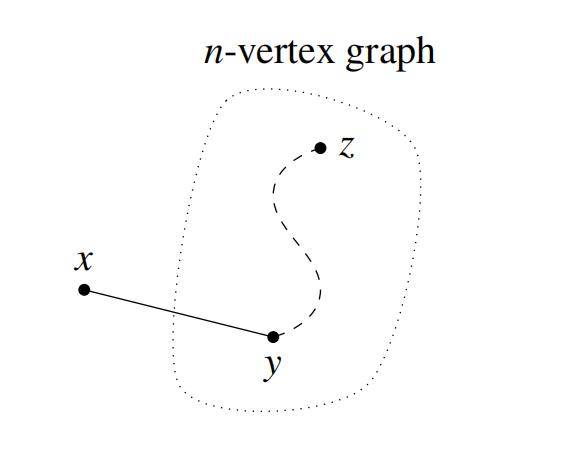
\includegraphics[width=0.5\textwidth]{graph4.png}

    All that remains is to check that there is a path from $x$ to every other vertex $z.$ Since $x$ has degree at least 1,there is an edge from $x$ to some other vertex; call it y. Thus, we can obtain a path from $x$ to $z$ by adjoining the edge $\{x,y\}$ to the path from y to z. This proves the claim for $n+1.$
\end{question}
\begin{solution}
    Consider this counterexample where $V=\{A,B,C,D\}$, $E=\{\{A,B\},\{C,D\}\}$

    The fundamental mistake here is that it only constructs an $(n+1)$-vertices graph that is connected but does not prove it true for any $(n+1)$-vertices graph. The proof demonstrates that build-up error can leads to a false proof applied to all natural number.
\end{solution}
\begin{question}
    \noindent
    (a) On the axis from San Francisco traffic habits to Los Angeles traffic habits, Old California is more towards San Francisco: that is, civilized. In Old California, all roads were one way streets. Suppose Old California had $n$ cities ($n \geq 2$) such that for every pair of cities $X$ and $Y$, either $X$ had a road to $Y$ or $Y$ had a road to $X$.
    
    Prove that there existed a city which was reachable from every other city by traveling through at most 2 roads.

    [Hint: Induction]\\
    (b) Consider a connected graph $G$ with $n$ vertices which has exactly $2m$ vertices of odd degree, where $m > 0$. Prove that there are $m$ walks that together cover all the edges of $G$ (i.e., each edge of $G$ occurs in exactly one of the $m$ walks, and each of the walks should not contain any particular edge more than once).

    [Hint: In lecture, we have shown that a connected undirected graph has an Eulerian tour if and only if every vertex has even degree. This fact may be useful in the proof.]\\
    (c) Prove that any graph $G$ is bipartite if and only if it has no tours of odd length.

    [Hint: In one of the directions, consider the lengths of paths starting from a given vertex.]
\end{question}
\begin{solution}
    \noindent
    (a) For $n=2$, it is trivial. Assume that the statement holds true for $n$ cities.
    For $(n+1)$ cities, remove a city $X$ and the roads connected to it so that there are $n$ cities and there exists at least one city $C$ that is reachable from every other city in at most 2 roads.
    Add $X$ and the roads back, if there exists a road from $X$ to a city that can reach $C$ in 1 road or a road from $X$ to $C$, then $C$ is still reachable from every other city in at most 2 roads.
    If it is not the case, then $X$ is at most 2 roads away from every other city.
    Therefore, we have proven that either $X$ or $C$ will be at most 2 roads away from every other city. \\
    (b) For 2 vertices of odd degree, we have proven that there exists a Eulerian walk from one odd-degree vertex to another.
    Assume that the statement holds true for $2m$ vertices of odd degree. 
    For $(2m+2)$ vertices of odd degree, find a path from one vertex of odd degree to another. The graph then splits into several connective components. 
    For each component, if there is no odd-degree vertex in it, then find a Eulerian tour from a vertex it shares with the path and make it a larger walk. 
    For other components, there exist no more than $2m$ vertices of odd degree, therefore we can find altogether $m$ walks from them to cover every other edge.
    Thus, we have found $(m+1)$ walks that together cover all the edges of $G$ with $(2m+2)$ vertices. Therefore, the statement holds true for all positive integer $m$.\\
    (c) Assume that $G$ is bipartite and it has tours of odd length, then it will take an odd number of steps to return to the starting point, which means that the starting point is in a different set from itself, which leads to contradiction.
    If $G$ has no tours of odd length, in any connective component, put all vertices that is an odd number of steps away from a raondom point $A$ to set $S$ and others to set $T$.
    Therefore, any two vertices connected to each other are not in the same set, which means G is bipartite.
\end{solution}
\section{Homework 03}
\begin{question}
    Let $G = (V, E)$ be an undirected graph with $|V| \geq 1$.\\
    (a) Prove that every connected component in an acyclic graph is a tree.\\
    (b) Suppose $G$ has $k$ connected components. Prove that if $G$ is acyclic, then $|E| = |V| - k$.\\
    (c) Prove that a graph with $|V|$ edges contains a cycle.
\end{question}
\begin{solution}
    \noindent
    (a) Every connected component in an acyclic graph is both connected and acyclic, therefore it is a tree by definition.\\
    (b) Let the $i$-th connected component has $v_i$ vertices.$|E|=\sum_1^k{\left( v_i-1 \right)}=\sum_1^k{v_i}-k=|V|-k$.\\
    (c) $|E|=|V|>|V|-k$, therefore at least one connected component contains a cycle, which means $G$ contains a cycle.
\end{solution}
\begin{question}
    In the lecture, you have seen that if $G$ is a hypercube of dimension $n$, then
    \begin{itemize}
        \item The vertices of $G$ are the binary strings of length $n$.
        \item $u$ and $v$ are connected by an edge if they differ in exactly one bit location.
    \end{itemize}

    A Hamiltonian tour of a graph is a sequence of vertices $v_0, v_1, \ldots, v_k$ such that:
    \begin{itemize}
        \item Each vertex appears exactly once in the sequence.
        \item Each pair of consecutive vertices is connected by an edge.
        \item $v_0$ and $v_k$ are connected by an edge.
    \end{itemize}
    (a) Show that a hypercube has an Eulerian tour if and only if $n$ is even.\\
    (b) Show that every hypercube has a Hamiltonian tour.
\end{question}
\begin{solution}
    \noindent
    (a) Any vertex in a $n$-dimensional hypercube has even degree if and only if $n$ is even, therefore a hypercube has an Eulerian tour if and only if $n$ is even.\\
    (b) For an 1-dimensional hypercube, it is trivial. Assume that every $n$-dimensional hypercube has a Hamiltonian tour.
    For an $(n+1)$-dimensional hypercube, in the $0x$ hypercube, start at a certain point and have a Hamiltonian tour, then take one step to the $1x$ hypercube, then make a same but backward Hamiltonian tour as in the $0x$ hypercube. The altogether sequence of vertices ia a Hamiltonian tour in an $(n+1)$-dimensional hypercube.
    Therefore, the statement holds true for any integer-dimensional hypercube.
\end{solution}
\begin{question}
    Let $G = (V,E)$ be an undirected graph. We define the complement of $G$ as $\overline{G} = (V,\overline{E})$ where $\overline{E} = \{(i,j) \mid i,j \in V, i \neq j\} - E$; that is, $\overline{G}$ has the same set of vertices as $G$, but an edge $e$ exists in $\overline{G}$ if and only if it does not exist in $G$.\\
    (a) Suppose $G$ has $v$ vertices and $e$ edges. How many edges does $\overline{G}$ have?\\
    (b) Prove that for any graph with at least 13 vertices, $G$ being planar implies that $\overline{G}$ is non-planar.\\
    (c) Now consider the converse of the previous part, i.e., for any graph $G$ with at least 13 vertices, if $\overline{G}$ is non-planar, then $G$ is planar. Construct a counterexample to show that the converse does not hold.

    Hint: Recall that if a graph contains a copy of $K_5$, then it is non-planar. Can this fact be used to construct a counterexample?
\end{question}
\begin{solution}
    \noindent
    (a) $\frac{v\left( v-1 \right)}{2}-e$.\\
    (b) $e\le 3v-6\Longrightarrow \frac{v\left( v-1 \right)}{2}-e\ge \frac{v\left( v-1 \right)}{2}-3v+6=\frac{v^2-7v+12}{2}>3v-6$.\\
    (c) Consider a graph with 13 vertices, where 5 of the vertices form a $K_5$ and no other edge exists.
\end{solution}
\end{document}